\providecommand{\main}{..}
\documentclass[\main/master.tex]{subfiles}
\begin{document}
\chapter{Methods and results}\label{chapter:Methods and results}

\section{System structure}
\subsection{Experiment setup}
\begin{figure}[htbp]
	\centering
	\fbox{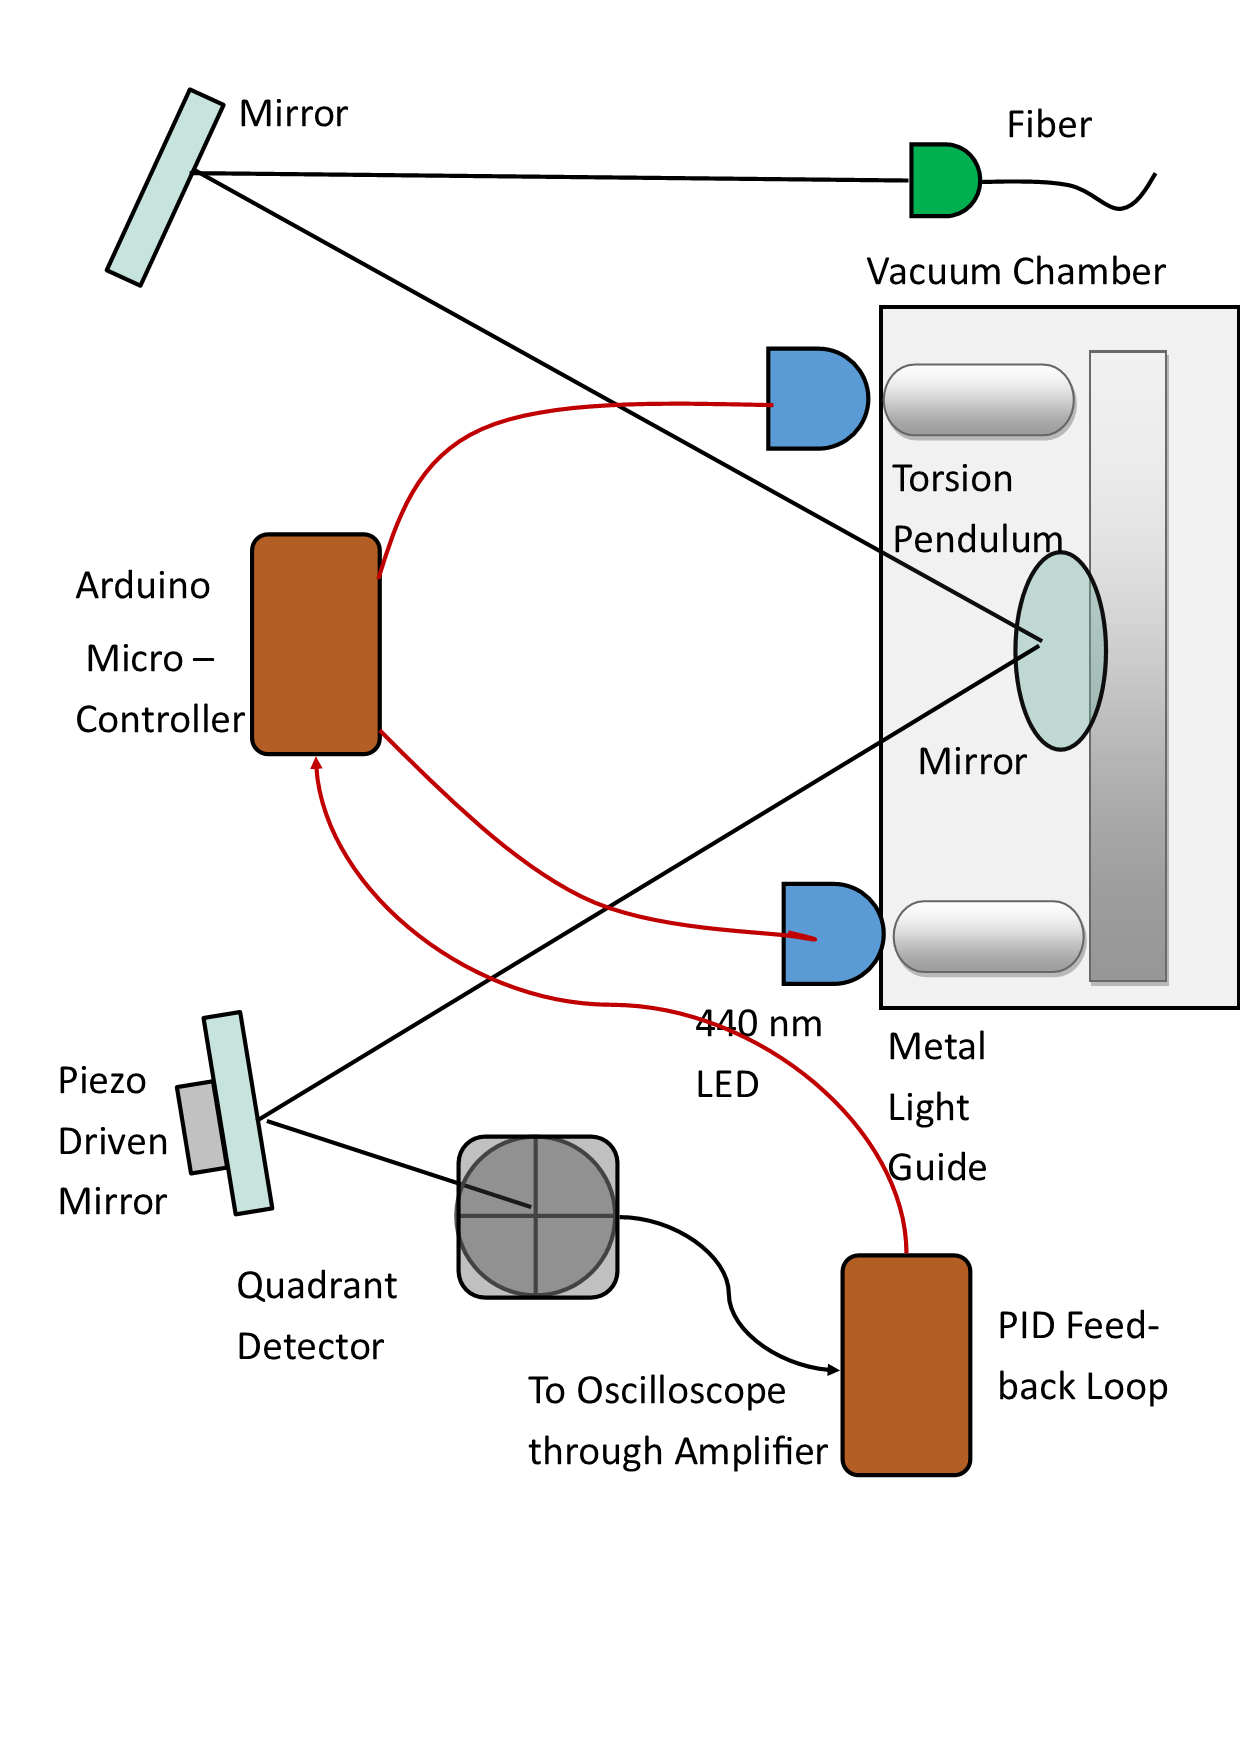
\includegraphics[scale=0.2]{\main/images/4 - methods and results/setup.png}}
	\caption[The experiment setup]{The experiment setup}
	\label{fig:setup}
\end{figure}
\FloatBarrier
\par\noindent
The experiment setup, shown in fig.~\ref{fig:setup}, is composed of a the torsion pendulum placed inside a vacuum chamber, a tilt angle measurement system and a feedback system. The experiment setup is placed inside a seismic box, which is not shown in the figure. The angle is measured by a laser beam deflected by the pendulum's front mirror and detected by a quadrant detector. The detector is connected to a computer by an oscilloscope through a signal amplifier. The light reflected from the pendulum mirror is reflected by a piezo driven mirror, which is tuned so that the reflected light would strike the detector's center (the PID needs a reference for error calculations). 
\par\noindent
The feedback system is composed of two LED light sources, modulated in real time by an Arduino micro-controller which is controlled by the PID feed-back loop in the computer. The LED light sources are placed in front of each of the transparent windows (viewports) on the sides of the vacuum chamber, each coupled to a side mass of the pendulum. 
\par\noindent
When the desired vacuum is achieved, the vacuum engine is disconnected using the valve and turned off, and the seismic box is closed. When the oscillations settle down to a level which could be affected by the weak torques caused by radiation pressure (an amplitude caused mainly by environmental noises, as explained in previous chapters). The angle is read in real time by the PID algorithm, and an equivalent radiation-pressure torque is exerted by the LED's flux damping down the pendulum noises.
\subsubsection{Design}
\begin{figure}[htbp]
	\centering
	\fbox{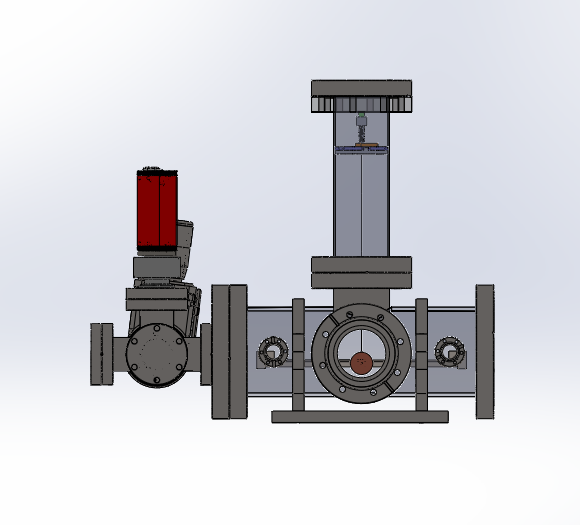
\includegraphics[scale=0.3]{\main/images/4 - methods and results/total_chamber.png}}
	\caption[Total chamber]{The system structure}
	\label{fig:Total chamber}
\end{figure}
\FloatBarrier
\par\noindent
The design of torsional pendulum and vacuum chamber, shown in fig.~\ref{fig:Total chamber}, was carried out using Solid Works. The design aims to minimize environment noises. As shown previously (eq.~\ref{eqn:heat conduction}, eq.~\ref{eqn:total_kinetic}, eq.~\ref{eqn:acoustic_intensity}, eq.~\ref{eqn:drag force}), Brownian motion of gas particles, thermal coupling, acoustic waves and friction are pressure dependent and are considerably reduced by maintaining low pressure. Therefore, the torsional pendulum is placed inside a vacuum chamber. Magnetic noise is reduced by choosing low magnetic permeability materials, avoiding capacitance and using a Faraday cage. 
\par\noindent
The vacuum chamber is placed inside seismic box, further reducing acoustic waves and magnetic noise. In order to maintain low pressure for long periods, the system is designed to minimize the outgassing rate by both, choosing low outgassing materials and avoiding air pockets inside the devices. 
\subsection{Torsional pendulum design}
\begin{figure}[htbp]
	\centering
	\fbox{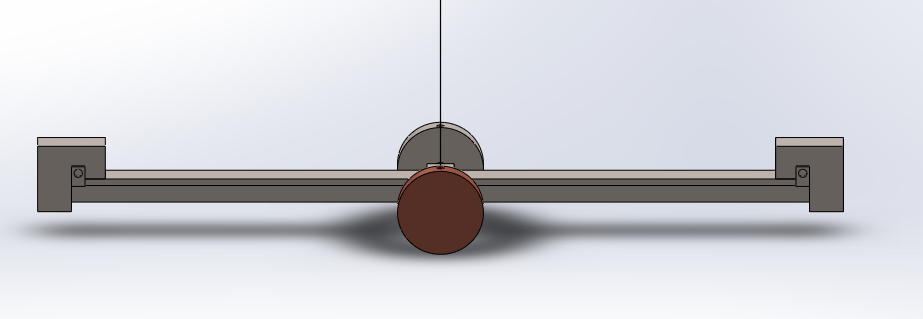
\includegraphics[scale=0.3]{\main/images/4 - methods and results/pendulum_front.png}}
	\caption[Torsional pendulum, front view]{Torsional pendulum, front view}
	\label{fig:pendulum front}
\end{figure}
\FloatBarrier
\par\noindent
The torsional pendulum design, shown in fig.~\ref{fig:pendulum front}, is composed of a thin rod with length $2l$, two identical masses $m$ on the sides, a front mirror and a balancing mass. The mirror is used for tilt angle measurement. Due to an unbalanced center of mass, the earth's gravity causes a downward torque $\tau_y$. 
\begin{figure}[htbp]
	\centering
	\fbox{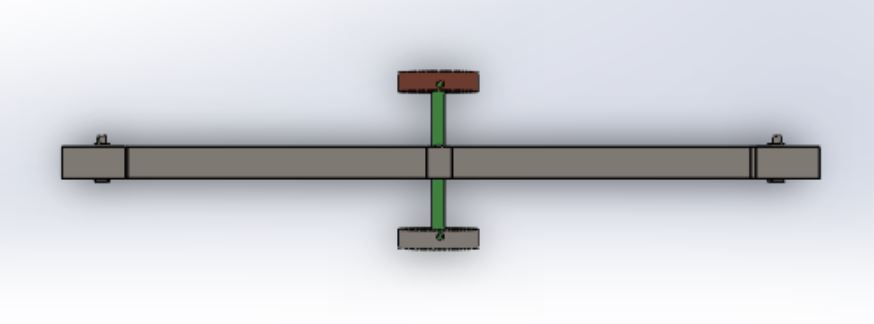
\includegraphics[scale=1.2]{\main/images/4 - methods and results/pendulum_top.JPG}}
	\caption[The torsional pendulum, top view]{The torsional pendulum, top view}
	\label{fig:pendulum top}
\end{figure}
\FloatBarrier 
\par\noindent
The center of mass is balanced using a balancing mass with similar shape and weight as the mirror, as shown in fig.~\ref{fig:pendulum top}. The balancing mass and the mirror are connected to the pendulum by a beam with length $w$ from their centers, and the downward torque is given by:
\begin{equation}
\tau_y = r_1\cdot m_1 g \cdot cos(0) - r_2\cdot m_2 g \cdot cos (0)\ = g( m_1 r_1  - m_2 (w-r_1) )  =0    \label{eqn:downward torque}
\end{equation}
Where $m_1$, $m_2$ are the masses of the mirror and the balancing mass, and $r_1$, $r_2$ are their distance from the pendulum's center of mass respectively. The beam allows to cancel out $\tau_y$ by accurate adjustment of the distance $r_1$, given by: 
\begin{equation}
 r_1 = \frac{w}{\frac{m_1}{m_2}+1}  \label{eqn:downward torque cancelled}
\end{equation}


\subsubsection{Design constraints}
\par\noindent
The chosen pendulum dimensions are designed to achieve large angle sensitivity to torque caused by a the gravity field (small string torsion coefficient $\kappa$ is needed, see eq.~\ref{eqn:theta average}) while maintaining large angle sensitivity to mass (longer oscillation time period $T$, see eq.~\ref{eqn:theta average}). For a torsional pendulum with moment of inertia $I$ and string torsion coefficient $\kappa$, the period $T$ is given by (eq.~\ref{eqn:undamped_omega}): 
\begin{equation}
T = 2\pi\sqrt{\frac{I}{\kappa}}= 2\pi\sqrt{\frac{2ml^2}{\kappa}} =  2\pi\sqrt{\frac{2ml^2}{\frac{G}{h} \frac{\pi d^4}{32}}}  \label{eqn:undamped_motion_equation_4}
\end{equation}
\par\noindent
As shown in eq.~\ref{eqn:undamped_motion_equation_4}, longer string $h$ with smaller diameter $d$ results in small string torsion coefficient while having a large period. A tungsten string is both, vacuum compatible (material with low outgassing) and has high tensile strength, which allows holding the pendulum robustly inside the vacuum chamber while having small string diameter. 
\par\noindent
In order to minimize the magnetic noise in the measurements, the torsional pendulum is made out of stainless steel 316 (instead of stainless steel 304) which has lower magnetic permeability \cite{SS316}, and the chosen front mirror is made fully of oxygen-free copper (OFC) instead of coated glass thus preventing capacitance. 
\subsubsection{Technical information}
The specifications of the designed elements of the system are:
\begin{easylist}
& Tungsten string;
&& made of 99.95\% pure Tungsten
&& length $h$ of 249 mm
&& diameter $d$ of 0.08 mm
&& shear modulus $G$ of 130-160 [Gpa]\cite{tungsten}.
& Torsional beam;
&& made of Stainless steel 316
&& length $2l$ of 218 mm
% && width of 10 mm 
%& & weight of 90 gram 
&& identical side masses weight $m$ of 20.5 gram
& Mirror;
&& made of oxygen-free copper (OFC), gold coated
&& diameter of 1 inch
\end{easylist}
\par\noindent
According to These specifications, the physical parameters of the torsional pendulum are:
\begin{easylist}
& expected;
&& $I = 0.487\cdot10^{-3}[kg\cdot m^2]$
&& $\kappa = 2.1\cdot10^{-6}[\frac{N\cdot m}{rad}] - 2.6\cdot10^{-6} [\frac{N\cdot m}{rad}]$
&& $T = 96[s] - 86 [s]$
& measured;
&& $\kappa = 2.7\cdot10^{-6}[\frac{N\cdot m}{rad}]$
&& $T = 86[s]$
\end{easylist}
\subsection{Vacuum chamber design}
\begin{figure}[htbp]
	\centering
	\fbox{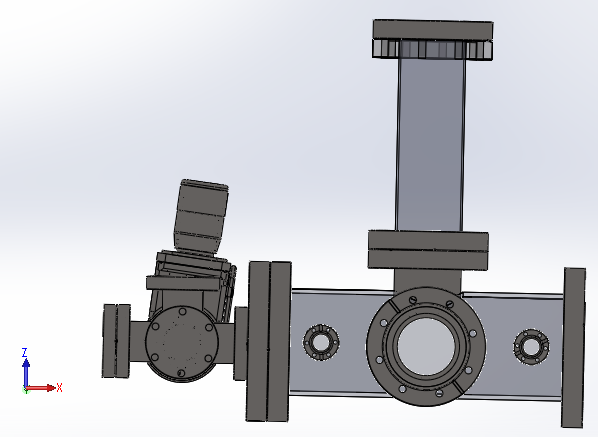
\includegraphics[scale=0.5]{\main/images/4 - methods and results/chamber_front.png}}
	\caption[Vacuum chamber, front view]{Vacuum chamber, front view}
	\label{fig:chamber front}
\end{figure}
\FloatBarrier

\par\noindent
The vacuum chamber, shown in fig.~\ref{fig:chamber front}, is composed of two cylindrical tubes placed one over the other with three view ports in front. The chamber is connected to a vacuum engine and gauge. The vacuum engine is connected to the chamber through a valve. The measurements are conducted when the valve is closed and the engine is off, to prevent rotation noise.

\subsubsection{Chamber viewports}
\par\noindent
The central viewport is located in front of the pendulum's front mirror. The central viewport has a 68.3mm view diameter where the mirror is located 82 mm away, giving a measurement FOV of about $39^0$ degrees. The other two small viewports are located in front of the pendulum's side masses and they are used for damping down the pendulum noises. They and are connected to the chamber through light guides. The view ports are transparent for light in 550-1100 nm range, with about 98$\%$ power transmittance in this range. 

\subsubsection{Pendulum mount}
\begin{figure}[htbp]
	\centering
	\fbox{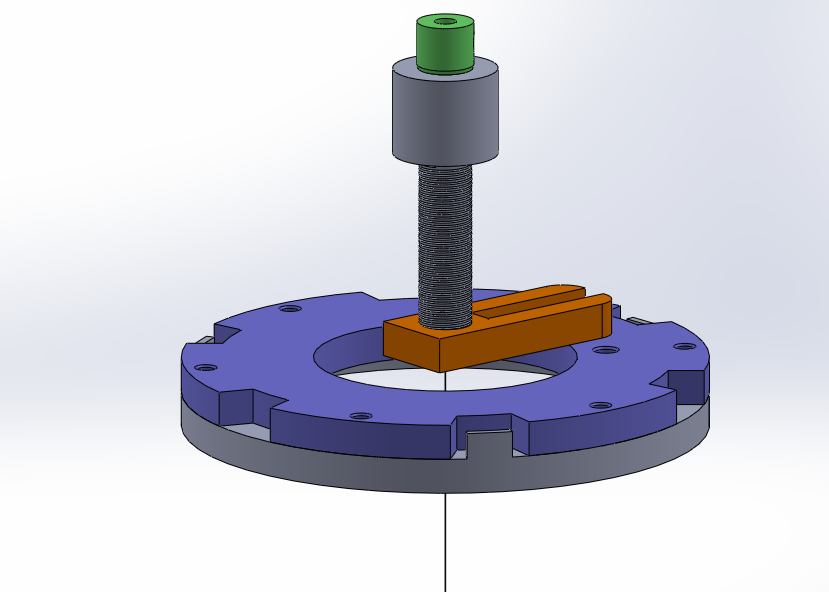
\includegraphics[scale=0.2]{\main/images/4 - methods and results/mount.png}}
	\caption[The pendulum mount]{The pendulum mount}
	\label{fig:mount}
\end{figure}
\FloatBarrier
\par\noindent
An adjustable mount is soldered to the upper tube of the chamber, as shown in fig.~\ref{fig:mount}. The string of the torsional pendulum is held by the mount, enabling the adjustment of the string's length and placing the pendulum in front of the viewports accurately. 
\subsubsection{Pressure increase}
\par\noindent
In this experiment, due to the measurement sensitivity, the vacuum engine pumping must be off during measurement. The main limitations to the maintenance of low pressure are the leakage $Q_L$ from the outside (eq.~\ref{eqn:leak rate}) and the outgassing $Q_{des}$ inside the chamber (eq.~\ref{eqn:desorption rate}), thus increase of the pressure at a constant rate over time. Due to the pendulum's shape and size, the vacuum chamber has large volume (high leak rate) and shell area (high outgassing rate).
\par\noindent
In order to minimize the pressure increase rate, the vacuum chamber is built using CF components which are designed for ultra high vacuum, and minimize the leak rate. Also, to reduce outgassing, the torsional pendulum and vacuum chamber were baked-out at $120 C^0$ for a week, using resistive wire. The achieved pressure for the experiments after cooling down is $P=1\cdot 10^{−4} [Hpa] - 5\cdot 10^{−3} [Hpa]$ for a month without pumping with the vacuum engine.

\subsection{Noise reduction}
As shown previously (eq.~\ref{eqn:heat conduction}, eq.~\ref{eqn:total_kinetic}, eq.~\ref{eqn:acoustic_intensity}, eq.~\ref{eqn:drag force}), Brownian motion of gas particles, thermal coupling, acoustic waves and friction are pressure dependent and are considerably reduced by maintaining low pressure.
I will add calculations..
\par\noindent
The measurement system is placed inside a seismic box which is also a Faraday cage with 76 mm thickness, that can block magnetic fields with frequencies $f \ge 30 [Hz]$ from the environment. Thus, the seismic box both reduces acoustic waves and magnetic noise from the environment.
\par\noindent
The vacuum chamber is a second cage that blocks magnetic noise from the electronic system placed inside the seismic box. The vacuum chambers is made out of approximately 3 mm thick stainless steel, blocking magnetic fields with frequencies $f\ge 20 [KHz]$ and reducing magnetic noise with lower frequencies.
\par\noindent
\subsubsection{Angle amplitude}
The initial measured angle due to to noises is $\theta_{max} = $

\section{Proportional–Integral–Derivative (PID)}

\subsection{Damped oscillator}
A PID feed-back loop is damping the torsional pendulum by continuously calculating the oscillator's error value from a defined set point, damping the error to zero. The PID mainly acts as friction, gradually working when the oscillations are at the maximum velocity slowing them down, with a torque $\tau_{PID}$ given by:
\begin{equation}
\tau_{PID}(t) = -\gamma\dot{e}(t) =  -\gamma\cdot [\dot{\theta}(t)-0]  =  -\gamma\dot{\theta}(t)  
\label{eqn:friction_torque_pid}
\end{equation}
Where $\gamma$ is the PID damping coefficient. When the defined set point is zero, the error $e(t)$ is the measured process which is the tilt angle of the torsional pendulum $\theta(t)$. The torque is modulated proportionately to the velocity of the oscillations, meaning it needs to have modulations with high speed compare to the oscillations period $T$ and high dynamic range compare to oscillations period $$.
\par\noindent
The torsional pendulum is a simple harmonic oscillator with maximal velocity $\dot{\theta}_{max} =\frac{2\pi}{T} \theta_{max} $ (see eq.~\ref{eqn:undamped_motion_equation_solved}). The PID damping coefficient $\gamma$ is a constant value given by:
\begin{equation}
\gamma  =  \frac{\tau_{PID}(t)}{\dot{\theta}(t)} = \frac{max(\tau_{PID})}{\dot{\theta}_{max}} =  \frac{max(\tau_{PID})}{\theta_{max}\cdot\frac{2\pi}{T}} =\frac{max(\tau_{PID})}{\theta_{max}}\cdot \frac{ T}{2\pi}          \label{eqn:damped_pid_motion_equation_2}
\end{equation}
As shown in eq.~\ref{eqn:damping_time} the damping time $\tau$ and damping ratio $\xi$ are given by:
\begin{equation}
\tau = \frac{T}{2 \pi \xi } =  \frac{2I}{\gamma} = \frac{\theta_{max}}{ max(\tau_{PID})} \cdot \frac{4\pi I}{T}  \label{eqn:damping_time_pid}
\end{equation}
The PID damping $\gamma$ and damping time $\tau$ depend on ratio between the initial oscillations angle and the maximal torque exerted by the PID. If the angle is too large compare to the external torque, the PID affect is negligible, causing an infinite damping time, meaning the torsional pendulum is extremely underdamped (very small $\xi$). The damping ratio $\xi$ when the pendulum is critically damped by $\tau_{critical}$ is given by (eq.~\ref{eqn:critically_damped_motion_equation}):
\begin{equation}
\xi = \frac{T^2}{ 8 \pi^2 I }\cdot\frac{ \tau_{critical}}{\theta_{max}} = 1 
\label{eqn:damping_ratio_pid}
\end{equation}
In order to critically damp the torsional pendulum by the PID, the PID torque $\tau_{PID}$ needs to be able to exert torques as large as the critical damping torque $max(\tau_{PID}) \geq  \tau_{critical}$. The maximal PID torque $max(\tau_{PID})$ is given by:
\begin{equation}
max(\tau_{PID}) \geq  \tau_{critical} = \frac{ 8 \pi^2 I }{T^2}\cdot\theta_{max} = \frac{ 8 \pi^2 \cdot 0.487\cdot10^{-3} }{(86)^2}\cdot 5\cdot10^{-6} = 2.6\cdot10^{-11}[N\cdot m]
\label{eqn:damping_torque_pid}
\end{equation}
The PID controlled torque $\tau_{PID}(t)$ needs to have modulations with high speed and high dynamic range to continuously damp the oscillations (eq.~\ref{eqn:friction_torque_pid}), and a maximal torque given by eq.~\ref{eqn:damping_torque_pid} to achieve critical damping.
\par\noindent


%The system is a damped oscillator with an external torque correction, shown in eq.~\ref{eqn:damped_motion_equation}.


\subsection{Radiation-pressure torque}
Two light sources with given flux, $\Theta_i$ cause radiation-pressure forces (eq.~\ref{eqn:radiation_force_power}), one on each mass of the torsional pendulum. As seen in eq.~\ref{eqn:net_gravitation_torque}, the difference between the two torques adds an external net torque. Assuming that both light fields have the same coupling efficiency $\eta$ and are very close to be perpendicular to the surface with negligible incidence angles $\alpha_1\approx\alpha_2\approx 0$, the radiation-pressure net torque is given by:  
\begin{equation}
\tau = l\cdot F_1 \cdot cos\alpha_1 - l\cdot F_2 \cdot cos\alpha_2\approx l(F_1 - F_2) \approx \frac{2l\eta}{{c}} \Delta \Theta \label{eqn:radiation torque}
\end{equation}
The radiation-pressure net torque is modulated by changing the difference between the light sources' flux (enabling high dynamic range to modulation), with maximal net torque $\tau_{max}$: 
\begin{equation}
\tau_{max}  \approx \frac{2l\eta}{{c}} \cdot 2 \Theta_{max} \approx \frac{0.218\cdot \eta}{{3\cdot10^{8}}} \cdot 2 \Theta_{max} \approx 7.27\cdot10^{-10} \cdot \eta\Theta_{max}   \label{eqn:max radiation torque}
\end{equation}
Where $\Theta_{max}$ is the is the the light sources' maximal flux with optical setup efficiency $\eta$. As shown in eq.~\ref{eqn:damping_torque_pid}, to successfully damp the torsional pendulum the maximal flux in each light source $\Theta_{max}$ is given by:
\begin{equation}
\Theta_{max} \geq \frac{2.6\cdot10^{-11}}{7.27\cdot10^{-10}\cdot \eta} \geq \frac{36\cdot10^{-3}}{\eta}
 \label{eqn:max radiation flux}
\end{equation}
\subsection{Laser setup}
Initially the modulated light sources were composed of a single laser #220 mW# diode coupled in series into two acousto optic modulators (AOM), with mod cleaning by coupling the modulated light into the torsional pendulum through optical fibers. An AOM can divide a single coherent light beam into two beams, with intensity ratio proportional to the AOM response to input voltage and short , resulting with a controlled modulation of the two light sources intensity.
\par\noindent
The setup minimized uncertainties of the light intensity since both light sources had a mutual source, causing a reduced torque uncertainty due to internal noises such as thermal and shot noise. The apparatus uncertainty due to the non linearity of the AOM response and laser power fluctuations proved to be larger than the uncertainties of the intensity difference. 
\subsubsection{Results}
\subsection{Arduino microcontroller}
Arduino is an inexpensive open-source microcontroller with a serial communication interface and a digital output without digital-to-analog converter (DAC). The Arduino Mega 2560 contains ATmega2560 8-bit controller, a $16 [MHz]$ crystal oscillator (clock) and 15 PWM outputs pins with digital output of $V_d = 5[V]$.
\subsubsection{Pulse Width Modulation}
\begin{figure}[htbp]
	\centering
	\fbox{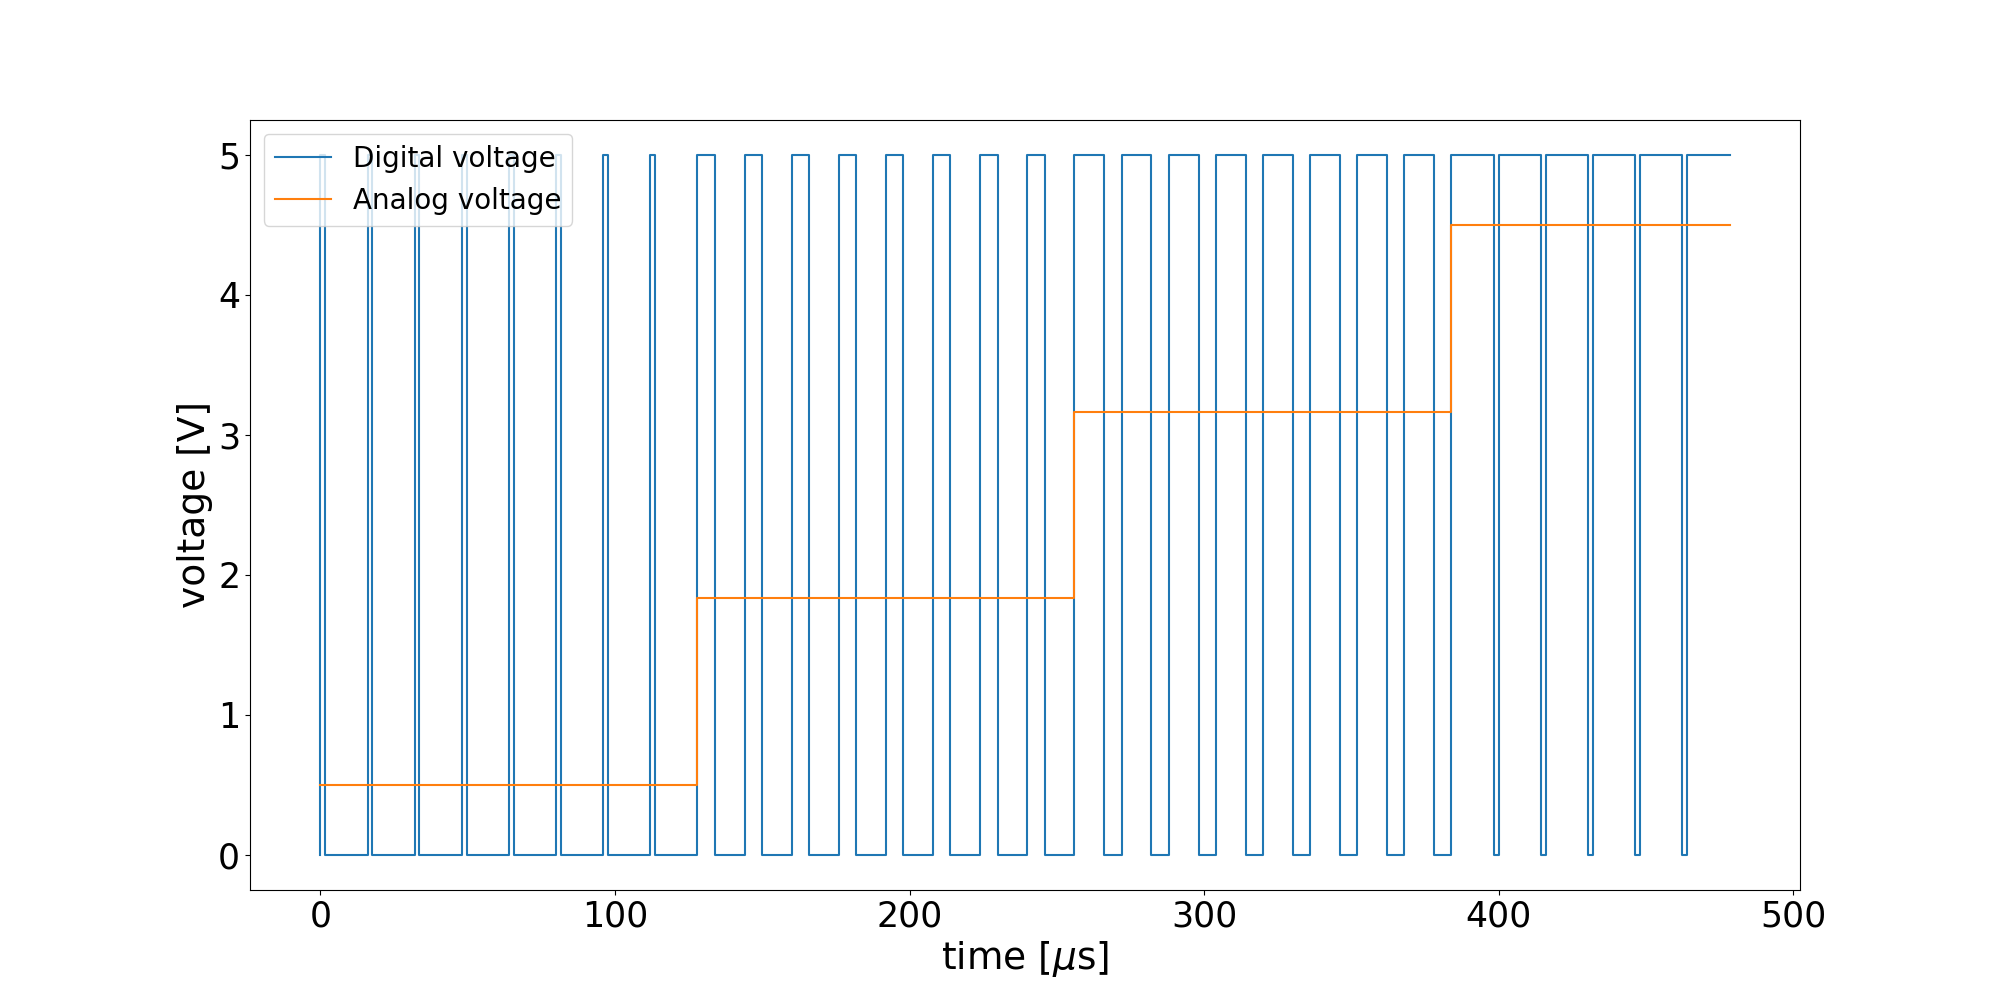
\includegraphics[scale=0.5]{\main/images/4 - methods and results/duty_cycle.png}}
	\caption[The PWM analog voltage]{The PWM analog voltage}
	\label{fig:duty_cycle}
\end{figure}
\FloatBarrier
\par\noindent
The microcontroller can simulate analog output using Pulse Width Modulation (PWM). As shown in fig.~\ref{fig:duty_cycle}, the controller switches the output signal fast between the digital output on and off, generating a square wave with period $T$. Pulse width ($PW$) is the time duration in which the signal is on. With the clock, the controller is able to modulate $PW$, changing the ratio of time signal is on compared to off, which is the duty cycle $D$:
\begin{equation}
D(t) = \frac{PW(t)}{T}\cdot 100  \label{eqn:duty cycle}
\end{equation}
The duty cycle varies between 0 to 100\%, with resolution limited by the controller. The Arduino is modulating the duty cycle, resulting in modulation of the The analog voltage (the average voltage) $V_a$ given by: 
\begin{equation}
V_a(t) = \frac{ PW(t)\cdot V_d}{ T}  = \frac{V_d}{100}\cdot D(t)  = \frac{5}{100}\cdot D(t)  \label{eqn:pwm voltage}
\end{equation}
Since the Arduino clock is connected to all PWM pins, they are all in sync. When all PWM pins have the same duty cycle, they all have the same voltage, frequency and phase. Even though the pins output vary in time, they are constant voltage supplies compare to each other, allowing to connect $N$ pins in parallel and increase the output current $I_{total}$ given by: 
\begin{equation}
I_{total} = N\cdot I   \label{eqn:pwm current}
\end{equation}
The clock is having about 120 full periods of the square wave before changing to a new duty cycle value, limiting the voltage modulation frequency. Also, in order to be able to change the duty cycle, the clock frequency is limited by the controller bit-rate. The PWM frequency is given by:
\begin{equation}
f_{PWM} = \frac{1 }{120T}= \frac{1 }{120 \frac{8-bit }{16MHz}}  \approx 500[Hz]	    \label{eqn:pwm frequency}
\end{equation}
\subsection{Light emitting diode (LED)}
The light emitting diode (LED) is a semiconductor based light source with high power, and a long lifetime. Forward voltage is applied to a p-n junction, causing electron injection and recombination with holes. The recombination is releasing energy in form of spontaneous emission photons (incoherent light). Due to the electrons life time before recombination, the LED could be modulated up to $100MHz$.
\par\noindent
The LED opening angle (FOV) varies between 45 to 120 degrees, and the emitted light is incoherent in width meaning it's hard to focus it to a point (not diffraction limited) and incoherent in length causing wide band spectrum. The LED current $I$ is defined by the Shockley diode equation for p-n junctions:
\begin{equation}
I  = I_s (e^{V_l\cdot \frac{e}{n k_B T} }-1) = I_s (e^{\frac{V_d}{n V_T} } -1) \overset{V_d>>V_T}{\approx} I_s e^{\frac{V_d}{n V_T} }   \label{eqn:led current}
\end{equation}
Where $I_s$ is the saturation current of the diode, $V_l$ is the LED forward voltage, $n$ is the led emission coefficient, $e$ is the electron charge, and $V_T$ is the thermal voltage. The LED forward voltage is given by:
\begin{equation}
V_l \approx n V_T ln10 log_{10} (\frac{I}{I_s}) \label{eqn:led voltage}
\end{equation}
\subsection{LED setup}
Since the forward voltage $V_l$ varies as the logarithm of the current, it varies slowly, being approximately constant over wide current range, resulting with large changes in the LED current due to small changes in the circuit supply voltage $V$. Driving circuit composed of resistor $R$ in series with the LED stabilizes the current, given by:
\begin{equation}
I =\frac{V-V_l}{R} \label{eqn:led circuit}
\end{equation}
The circuit is composed of a blue LED with $V_l\approx 4.5V$, supply voltage with 6 parallel PWM Arduino pins (eq.~\ref{eqn:pwm current}, eq.~\ref{eqn:pwm voltage}) and resistor $R = 200\Omega$, the LED radiant flux $[W]$ is given by:
\begin{equation}
\Theta(t) = I_{total}\cdot V_l = NI\cdot V_l = N V_l \frac{V-V_l}{R}\cdot  =N V_l\frac{\frac{5}{100}\cdot D(t)-V_l}{R} \approx N V_l\frac{\frac{5}{100}\cdot D(t)}{R} = 0.007\cdot D(t)\label{eqn:led power}
\end{equation}
\par\noindent
In order to overcome the led uncoherent profile and large FOV, the light is coupled to a light guide, a pipe made of thin filaments causing internal reflections used  to illuminate small areas, regardless of the spectral characteristics of the light source. Light guide mainly depend on the entrance and exit cross section and length, making it ideal to overcome focusing problems. 
\par\noindent
Due to coupling efficiency and size difference between the output beam from the lightguide and the pendulum sides, the efficiency of flux hitting the pendulum is estimated to be $\eta = 0.7$ and the torque $\tau(t)_{LED}$ is given by:
\begin{equation}
\tau(t)_{LED}  =\frac{2l\eta}{{c}} (\Theta_1(t) -\Theta_2(t)) = 3.56^{-12}(D_1(t) -D_2(t)) 
\label{eqn:led torque}
\end{equation}
\par\noindent
The LED power could be approximated by linear approximation of the Arduino duty cycle $D(t)$, which varies between 0 to 100\% with 8bit resolution, generating torques up to $\tau = 7\cdot10^-{10} [N\cdot m]$ with modulation steps of $\Delta\tau = 1.4\cdot10^-{12} [N\cdot m]$. As shown in eq.~\ref{eqn:pwm frequency}), the LED could be modulated up to $500[Hz]$ resulting with fast modulated external force for the PID algorithm. Also, since the led power could be approximated using linear approximation, it allows to control the approximated power output by changing the PID gain values.  
  


\subsection{Control stability}
PID control does not guarantee optimal control or stability, the control system aims to reach the desired set point by critically damping of the process (the oscillator). Well tuned control reaches the desired set point fast and accurate, and able to resist external forces trying to move the process from the set point.
\par\noindent
Overshoot is when output signal or function exceeds the target value. The response signal is not accurate compare to target. In control theory there are two wanted conflicting properties; an accurate response (small overshoot), and small risetime (fast response). Overshoot is usually measured in percentage overshoot (PO). For second order systems, such as damped oscillators PO is given by:
\begin{equation}
PO = 100\cdot e ^{\frac{-\xi\pi}{\sqrt{1-\xi^2}}} = \frac{output-target}{target}   \label{eqn:percentage_overshoot}
\end{equation}
\par\noindent
The controller response to error (shown in eq.~\ref{eqn:PID response}) defines how much will the oscillator overshoot the setpoint. When controller gains  are too high, instead of critical damping there is overdamping causing overshoot. Due to the high gains the overshoot response overshoots again to the other side, causing the system to be driven (shown in eq.~\ref{eqn:driven_motion_equation_2}).

\section{pid operate (algorithm and measurement)}
\subsection{Accuracy}


\end{document}